\section*{Experimental Results}

This section details the experimental setup and evaluation of SaltNet's denoising performance in comparison to existing state-of-the-art methods. We conducted a comprehensive evaluation across various noise types, noise levels, and benchmark datasets.

\subsection{Datasets}

The performance of SaltNet was evaluated on four public datasets \textbf{BSD68}\cite{Martin01}, \textbf{Kodak24}\cite{Kodak}, \textbf{Urban100}\cite{Huang2015}, and \textbf{Set12}\cite{Set12}.

\subsection{Noise Simulation and Levels}

Images from the four utilized datasets were corrupted with one of four distinct types of noise: \textbf{Poisson Noise}, \textbf{Bernoulli Noise}, and \textbf{Salt and Pepper Noise} with noise density ranging from 150/255 to 240/255 in increments of 10/255. And \textbf{Gaussian Noise}: with noise levels (standard deviation $\sigma$) were set to 15/255, 25/255, 50/255, and 60/255.

Detailed experimental results of SaltNet for each dataset and noise type are listed. Followed by a comparison with a locally trained Restormer version. This Restormer version was trained following the exactly the same methods and data detailed in \ref{sec:training_details}. The denoising performance was quantitatively evaluated using the \textbf{Peak Signal-to-Noise Ratio (PSNR)} and \textbf{Structural Similarity Index (SSIM)} metrics. PSNR focusing on pixel-level fidelity and SSIM emphasizing structural and perceptual aspects.

SaltNet's denoising performance is very competitive with Restormer's when the trained using the same method.
\subsection{Quantitative Results}
\subsubsection{Gaussian Noise}

\begin{table}[!hbt]
    \centering
    \begin{minipage}{0.48\textwidth} % Adjust width as needed
        \centering
        \begin{tabular}{ccccc}
            \hline
            & \multicolumn{4}{c}{Gaussian Noise Density} \\
            & 15 & 25 & 50 & 60 \\
            \hline
            Average & 31.38 & 29.08 & 25.99 & 25.19 \\
            \hline
            BSD68 & 31.28 & 29.05 & 26.19 & 25.48 \\
            Kodak24 & 32.27 & 30.21 & 27.46 & 26.74 \\
            Set 12 & 32.43 & 30.23 & 27.12 & 26.33 \\
            Urban100 & 31.10 & 28.69 & 25.36 & 24.48 \\        
            \hline
        \end{tabular}
        \caption{SaltNet - Bernoulli Detailed PSNR Results}
    \end{minipage}
    \hfill
    \vline
    \begin{minipage}{0.45\textwidth}
        \centering
        \begin{tabular}{cccc}
            \hline
            \multicolumn{4}{c}{Gaussian Noise Density} \\
            15 & 25 & 50 & 60 \\
            \hline
            0.9057 & 0.8566 & 0.7560 & 0.7242 \\
            \hline
            0.8893 & 0.8300 & 0.7192 & 0.6869 \\
            0.8865 & 0.8327 & 0.7342 & 0.7070 \\
            0.9001 & 0.8611 & 0.7830 & 0.7583 \\
            0.9221 & 0.8798 & 0.7831 & 0.7497 \\
            \hline
        \end{tabular}
        \caption{SaltNet - Bernoulli Detailed SSIM Results}
    \end{minipage}
    \end{table}

\begin{table}[!hbt]
    \centering
    \begin{tabular}{ccccc}
        \hline
        Alpha & \multicolumn{2}{c}{AVG. PSNR} & \multicolumn{2}{c}{AVG. SSIM} \\
            & SaltNet & Restormer & SaltNet & Restormer \\
        \hline
        15    & \underline{31.38}   & 31.05     & 0.9057  & \underline{0.9075}  \\
        25    & \underline{29.08}   & 28.87     & \underline{0.8566}  & 0.8562  \\
        50    & \underline{25.99}   & 25.76     & \underline{0.7560}  & 0.7500  \\
        60    & \underline{25.19}   & 24.96     & \underline{0.7242}  & 0.7166  \\
        \hline
    \end{tabular}
    \caption{Gaussian Noise SaltNet vs. Restormer Comparison}
\end{table}

% \subsubsection{Gaussian Noise}


\begin{table}[!hbt]
    \centering
    \begin{tabular}{ccccc}
        \hline
        & \multicolumn{4}{c}{Gaussian Noise Density} \\
        & 15 & 25 & 50 & 60 \\
        \hline
        Average & 31.38 & 29.08 & 25.99 & 25.19 \\
        \hline
        BSD68 & 31.28 & 29.05 & 26.19 & 25.48 \\
        Kodak24 & 32.27 & 30.21 & 27.46 & 26.74 \\
        Set 12 & 32.43 & 30.23 & 27.12 & 26.33 \\
        Urban100 & 31.10 & 28.69 & 25.36 & 24.48 \\        
        \hline
    \end{tabular}
    \caption{SaltNet Detailed PSNR Gaussian Noise Results}
\end{table}

\begin{table}[!hbt]
    \centering
    \begin{tabular}{ccccc}
        \hline
        & \multicolumn{4}{c}{Gaussian Noise Density} \\
        & 15 & 25 & 50 & 60 \\
        \hline
        Average & 0.9057 & 0.8566 & 0.7560 & 0.7242 \\
        \hline
        BSD68 & 0.8893 & 0.8300 & 0.7192 & 0.6869 \\
        Kodak24 & 0.8865 & 0.8327 & 0.7342 & 0.7070 \\
        Set12 & 0.9001 & 0.8611 & 0.7830 & 0.7583 \\
        Urban100 & 0.9221 & 0.8798 & 0.7831 & 0.7497 \\
        \hline
    \end{tabular}
    \caption{SaltNet Detailed SSIM Gaussian Noise Results}
\end{table}

\begin{table}[!hbt]
    \centering
    \begin{tabular}{ccccc}
        \hline
        Alpha & \multicolumn{2}{c}{AVG. PSNR} & \multicolumn{2}{c}{AVG. SSIM} \\
            & SaltNet & Restormer & SaltNet & Restormer \\
        \hline
        15    & \underline{31.38}   & 31.05     & 0.9057  & \underline{0.9075}  \\
        25    & \underline{29.08}   & 28.87     & \underline{0.8566}  & 0.8562  \\
        50    & \underline{25.99}   & 25.76     & \underline{0.7560}  & 0.7500  \\
        60    & \underline{25.19}   & 24.96     & \underline{0.7242}  & 0.7166  \\
        \hline
    \end{tabular}
    \caption{Gaussian Noise SaltNet vs. Restormer Comparison}
\end{table}


\subsubsection{Bernoulli Noise}

\begin{table}[!hbt]
    \centering
    \begin{tabular}{ccccccccccc}
        \hline
        & \multicolumn{10}{c}{Bernoulli Noise Density} \\
        & 150 & 160 & 170 & 180 & 190 & 200 & 210 & 220 & 230 & 240 \\
        \hline
        Average & 30.10 & 29.48 & 28.84 & 28.15 & 27.43 & 26.64 & 25.78 & 24.81 & 23.61 & 22.06 \\
        \hline
        BSD68 & 30.83 & 30.17 & 29.58 & 28.92 & 28.26 & 27.55 & 26.78 & 25.93 & 24.90 & 23.58 \\
        Kodak24 & 30.78 & 30.33 & 29.88 & 29.39 & 28.85 & 28.29 & 27.61 & 26.89 & 25.93 & 24.69 \\
        Set 12 & 32.04 & 31.39 & 30.80 & 30.17 & 29.37 & 28.49 & 27.58 & 26.64 & 25.25 & 23.45 \\
        Urban100 & 29.21 & 28.57 & 27.84 & 27.08 & 26.30 & 25.40 & 24.44 & 23.33 & 21.97 & 20.23 \\
        \hline
    \end{tabular}
    \caption{SaltNet - Bernoulli Detailed PSNR Results}
\end{table}

\begin{table}[!hbt]
    \centering
    \begin{tabular}{ccccccccccc}
        \hline
        & \multicolumn{10}{c}{Bernoulli Noise Density} \\
        & 150 & 160 & 170 & 180 & 190 & 200 & 210 & 220 & 230 & 240 \\
        \hline
        Average & 0.9304 & 0.9208 & 0.9097 & 0.8964 & 0.8803 & 0.8600 & 0.8346 & 0.8001 & 0.7502 & 0.6709 \\
        \hline
        BSD68 & 0.9164 & 0.9043 & 0.8912 & 0.8758 & 0.8576 & 0.8358 & 0.8096 & 0.7757 & 0.7307 & 0.6643 \\
        Kodak24 & 0.9310 & 0.9214 & 0.9106 & 0.8976 & 0.8819 & 0.8636 & 0.8405 & 0.8110 & 0.7707 & 0.7108 \\
        Set 12 & 0.9435 & 0.9367 & 0.9286 & 0.9187 & 0.9064 & 0.8920 & 0.8721 & 0.8477 & 0.8092 & 0.7473 \\
        Urban100 & 0.9382 & 0.9300 & 0.9198 & 0.9075 & 0.8921 & 0.8717 & 0.8457 & 0.8082 & 0.7514 & 0.6567 \\
        \hline
    \end{tabular}
    \caption{SaltNet - Bernoulli Detailed SSIM Results}
\end{table}

\begin{table}[!hbt]
    \centering
    \begin{tabular}{ccccc}
        \hline
        Bernoulli & \multicolumn{2}{c}{AVG. PSNR} & \multicolumn{2}{c}{AVG. SSIM} \\
        Noise Density & SaltNet & Restormer & SaltNet & Restormer \\
        \hline
        150 & \underline{30.10} & 29.84 & 0.9304 & \underline{0.9307} \\
        160 & \underline{29.48} & 29.25 & 0.9208 & \underline{0.9215} \\
        170 & \underline{28.84} & 28.65 & 0.9097 & \underline{0.9104} \\
        180 & \underline{28.15} & 28.00 & 0.8964 & \underline{0.8974} \\
        190 & \underline{27.43} & 27.31 & 0.8803 & \underline{0.8815} \\
        200 & \underline{26.64} & 26.56 & 0.8600 & \underline{0.8620} \\
        210 & \underline{25.78} & 25.75 & 0.8346 & \underline{0.8365} \\
        220 & \underline{24.81} & 24.80 & 0.8001 & \underline{0.8026} \\
        230 & 23.61 & \underline{23.65} & 0.7502 & \underline{0.7542} \\
        240 & 22.06 & \underline{22.19} & 0.6709 & \underline{0.6795} \\
        \hline
    \end{tabular}
    \caption{Bernoulli Noise SaltNet vs. Restormer Comparison}
\end{table}

\subsubsection{Poisson Noise}


\begin{table}[!hbt]
    \centering
    \begin{tabular}{ccccccccccc}
        \hline
        & \multicolumn{10}{c}{Poisson Noise Density} \\
        & 150 & 160 & 170 & 180 & 190 & 200 & 210 & 220 & 230 & 240 \\
        \hline
        Average & 31.48 & 31.19 & 30.99 & 30.83 & 30.58 & 30.34 & 30.16 & 30.00 & 29.79 & 29.54 \\
        \hline
        BSD68 & 31.95 & 31.64 & 31.48 & 31.30 & 31.03 & 30.89 & 30.65 & 30.52 & 30.37 & 30.11 \\
        Kodak24 & 33.76 & 33.34 & 33.19 & 32.94 & 32.76 & 32.53 & 32.39 & 32.21 & 31.96 & 31.75 \\
        Set12 & 34.26 & 34.08 & 33.75 & 33.55 & 33.28 & 33.08 & 32.81 & 32.69 & 32.35 & 32.17 \\
        Urban100 & 30.27 & 30.03 & 29.80 & 29.69 & 29.43 & 29.12 & 28.97 & 28.79 & 28.57 & 28.31 \\
        \hline
    \end{tabular}
    \caption{SaltNet - Poisson Detailed PSNR Results}
\end{table}

\begin{table}[!hbt]
    \centering
    \begin{tabular}{ccccccccccc}
        \hline
        & \multicolumn{10}{c}{Poisson Noise Density} \\
        & 150 & 160 & 170 & 180 & 190 & 200 & 210 & 220 & 230 & 240 \\
        \hline
        Average & 0.9491 & 0.9460 & 0.9438 & 0.9408 & 0.9372 & 0.9328 & 0.9302 & 0.9263 & 0.9232 & 0.9170 \\
        \hline
        BSD68 & 0.9433 & 0.9396 & 0.9371 & 0.9330 & 0.9301 & 0.9260 & 0.9220 & 0.9183 & 0.9151 & 0.9081 \\
        Kodak24 & 0.9648 & 0.9593 & 0.9583 & 0.9549 & 0.9513 & 0.9478 & 0.9451 & 0.9413 & 0.9380 & 0.9301 \\
        Set12 & 0.9748 & 0.9737 & 0.9721 & 0.9701 & 0.9678 & 0.9647 & 0.9636 & 0.9625 & 0.9590 & 0.9567 \\
        Urban100 & 0.9462 & 0.9438 & 0.9415 & 0.9391 & 0.9350 & 0.9299 & 0.9283 & 0.9239 & 0.9209 & 0.9152 \\
        \hline
    \end{tabular}
    \caption{SaltNet - Poisson Detailed SSIM Results}
\end{table}

\begin{table}[!hbt]
    \centering
    \begin{tabular}{ccccc}
        \hline
        Poisson & \multicolumn{2}{c}{AVG. PSNR} & \multicolumn{2}{c}{AVG. SSIM} \\
        Noise Density & SaltNet & Restormer & SaltNet & Restormer \\
        \hline
        150 & \underline{31.48} & 30.15 & 0.9491 & \underline{0.9512} \\
        160 & \underline{31.19} & 29.96 & 0.9460 & \underline{0.9482} \\
        170 & \underline{30.99} & 29.79 & 0.9438 & \underline{0.9459} \\
        180 & \underline{30.83} & 29.63 & 0.9408 & \underline{0.9429} \\
        190 & \underline{30.58} & 29.45 & 0.9372 & \underline{0.9404} \\
        200 & \underline{30.34} & 29.30 & 0.9328 & \underline{0.9376} \\
        210 & \underline{30.16} & 29.19 & 0.9302 & \underline{0.9352} \\
        220 & \underline{30.00} & 29.05 & 0.9263 & \underline{0.9328} \\
        230 & \underline{29.79} & 28.99 & 0.9232 & \underline{0.9303} \\
        240 & \underline{29.54} & 28.86 & 0.9170 & \underline{0.9277} \\
        \hline
    \end{tabular}
    \caption{Poisson Noise SaltNet vs. Restormer Comparison}
\end{table}

\subsubsection{Salt \& Pepper Noise}


\begin{table}[!hbt]
    \centering
    \begin{tabular}{ccccccccccc}
        \hline
        & \multicolumn{10}{c}{Salt \& Pepper Noise Density} \\
        & 150 & 160 & 170 & 180 & 190 & 200 & 210 & 220 & 230 & 240 \\
        \hline
        Average & 29.87 & 29.27 & 28.64 & 27.97 & 27.25 & 26.49 & 25.62 & 24.65 & 23.47 & 21.90 \\
        \hline
        BSD68 & 30.68 & 30.10 & 29.49 & 28.85 & 28.17 & 27.49 & 26.71 & 25.84 & 24.85 & 23.47 \\
        Kodak24 & 30.54 & 30.11 & 29.67 & 29.17 & 28.65 & 28.10 & 27.42 & 26.69 & 25.80 & 24.52 \\
        Set12 & 32.04 & 31.40 & 30.79 & 30.02 & 29.26 & 28.48 & 27.68 & 26.50 & 25.22 & 23.50 \\
        Urban100 & 28.89 & 28.24 & 27.55 & 26.84 & 26.06 & 25.19 & 24.19 & 23.12 & 21.76 & 20.01 \\
        \hline
    \end{tabular}
    \caption{SaltNet - Detailed PSNR Salt \& Pepper Results}
\end{table}

\begin{table}[!hbt]
    \centering
    \begin{tabular}{ccccccccccc}
        \hline
        & \multicolumn{10}{c}{Salt \& Pepper Noise Density} \\
        & 150 & 160 & 170 & 180 & 190 & 200 & 210 & 220 & 230 & 240 \\
        \hline
        Average & 0.9293 & 0.9197 & 0.9085 & 0.8949 & 0.8785 & 0.8585 & 0.8322 & 0.7970 & 0.7471 & 0.6664 \\
        \hline
        BSD68 & 0.9152 & 0.9037 & 0.8903 & 0.8747 & 0.8561 & 0.8347 & 0.8076 & 0.7734 & 0.7287 & 0.6617 \\
        Kodak24 & 0.9293 & 0.9198 & 0.9086 & 0.8954 & 0.8797 & 0.8613 & 0.8375 & 0.8074 & 0.7676 & 0.7068 \\
        Set12 & 0.9431 & 0.9358 & 0.9278 & 0.9175 & 0.9053 & 0.8913 & 0.8721 & 0.8462 & 0.8080 & 0.7466 \\
        Urban100 & 0.9373 & 0.9287 & 0.9184 & 0.9059 & 0.8902 & 0.8700 & 0.8428 & 0.8047 & 0.7473 & 0.6502 \\
        \hline
    \end{tabular}
    \caption{SaltNet - Detailed SSIM Salt \& Pepper Results}
\end{table}

\begin{table}[!hbt]
    \centering
    \begin{tabular}{ccccc}
        \hline
        Salt \& Pepper & \multicolumn{2}{c}{AVG. PSNR} & \multicolumn{2}{c}{AVG. SSIM} \\
        Noise Density & SaltNet & Restormer & SaltNet & Restormer \\
        \hline
        150 & \underline{29.87} & 29.27 & \underline{0.9293} & 0.9278 \\
        160 & \underline{29.27} & 28.71 & \underline{0.9197} & 0.9182 \\
        170 & \underline{28.64} & 28.10 & \underline{0.9085} & 0.9070 \\
        180 & \underline{27.97} & 27.52 & \underline{0.8949} & 0.8938 \\
        190 & \underline{27.25} & 26.87 & \underline{0.8785} & 0.8775 \\
        200 & \underline{26.49} & 26.17 & \underline{0.8585} & 0.8571 \\
        210 & \underline{25.62} & 25.32 & \underline{0.8322} & 0.8311 \\
        220 & \underline{24.65} & 24.41 & \underline{0.7970} & 0.7968 \\
        230 & \underline{23.47} & 23.31 & 0.7471 & \underline{0.7477} \\
        240 & \underline{21.90} & \underline{21.90} & 0.6664 & \underline{0.6704} \\
        \hline
    \end{tabular}
    \caption{Salt \& Pepper Noise SaltNet vs. Restormer Comparison}
\end{table}

\subsection{Qualitative Results and Visual Inspection}

Below are some samples of our experimentation. Full results are in the Resources Section\ref{sec:resources}

\begin{figure}[htpb]
    \centering
    \begin{subfigure}{0.48\textwidth}
        \centering
        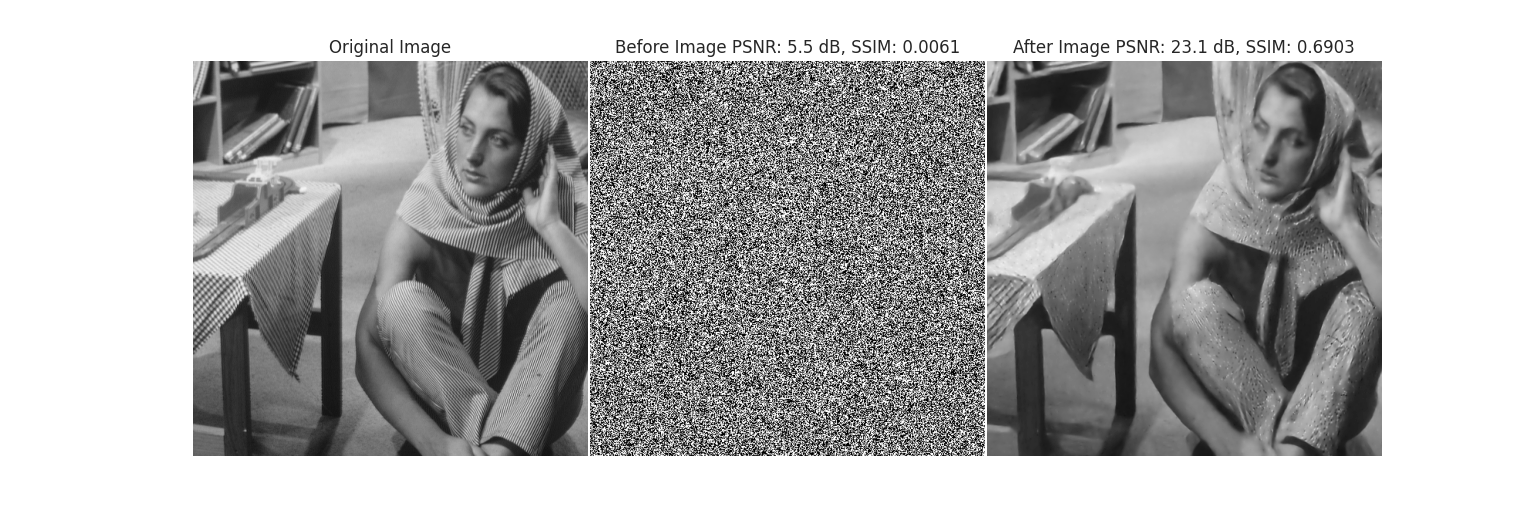
\includegraphics[width=\textwidth]{assets/240_sap_saltnet.png}
        \caption{SaltNet (Salt \& Pepper, 240/250)}
    \end{subfigure}
    \hfill
    \begin{subfigure}{0.48\textwidth}
        \centering
        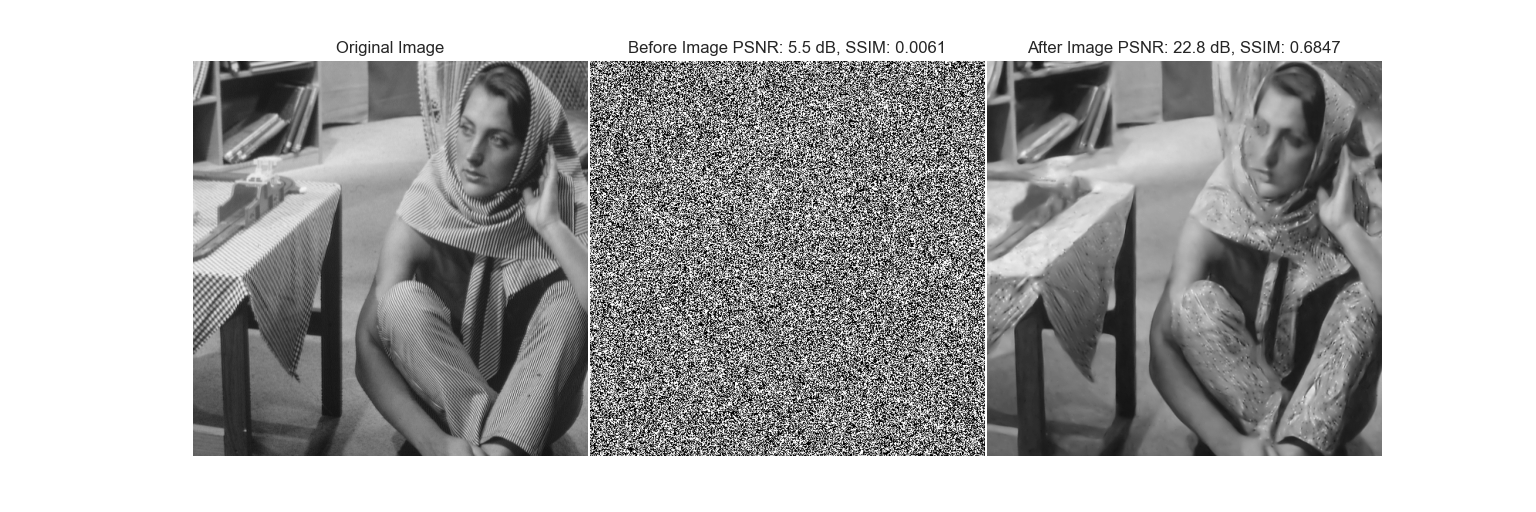
\includegraphics[width=\textwidth]{assets/240_sap_restormer.png}
        \caption{Restormer (Salt \& Pepper, 240/250)}
    \end{subfigure}
    \begin{subfigure}{0.48\textwidth}
        \centering
        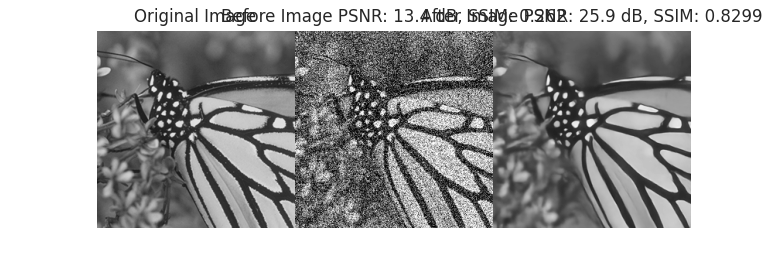
\includegraphics[width=\textwidth]{assets/60_gau_2_saltnet.png}
        \caption{SaltNet (Gaussian, 60/250)}
    \end{subfigure}
    \hfill
    \begin{subfigure}{0.48\textwidth}
        \centering
        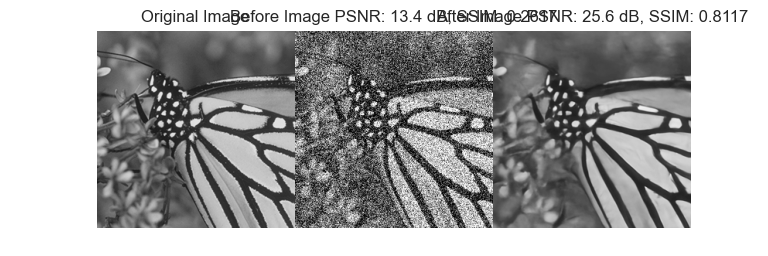
\includegraphics[width=\textwidth]{assets/60_gau_2_restormer.png}
        \caption{Restormer (Gaussian, 60/250)}
    \end{subfigure}
    \begin{subfigure}{0.48\textwidth}
        \centering
        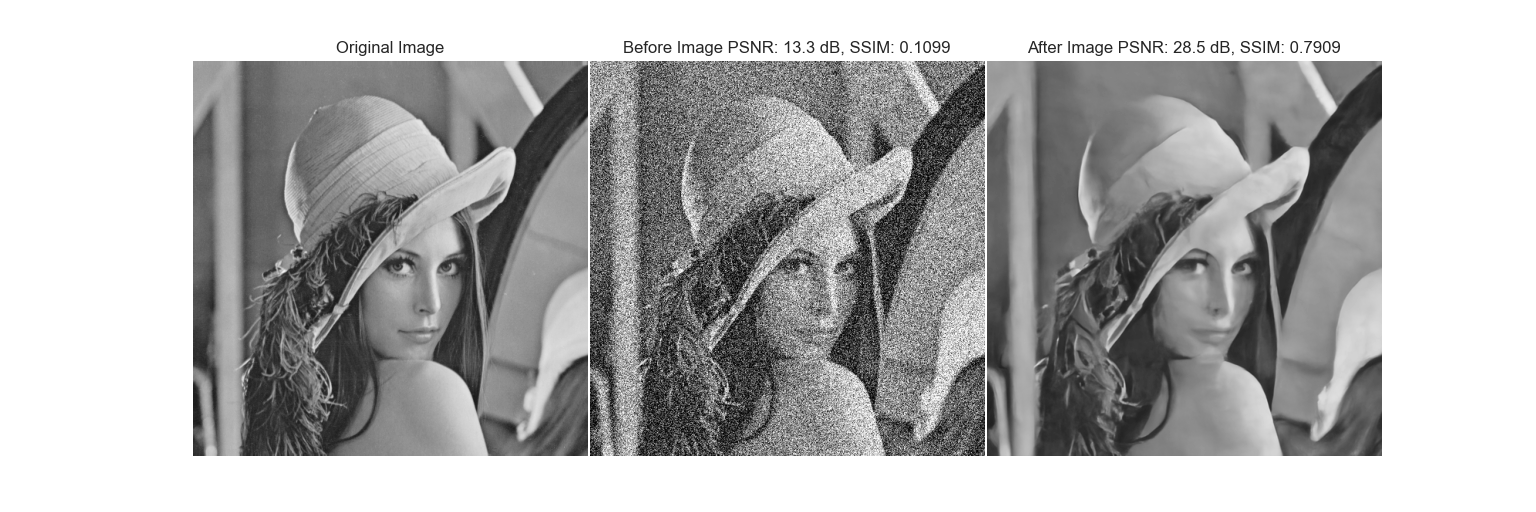
\includegraphics[width=\textwidth]{assets/60_gau_saltnet.png}
        \caption{SaltNet (Gaussian, 60/250)}
    \end{subfigure}
    \hfill
    \begin{subfigure}{0.48\textwidth}
        \centering
        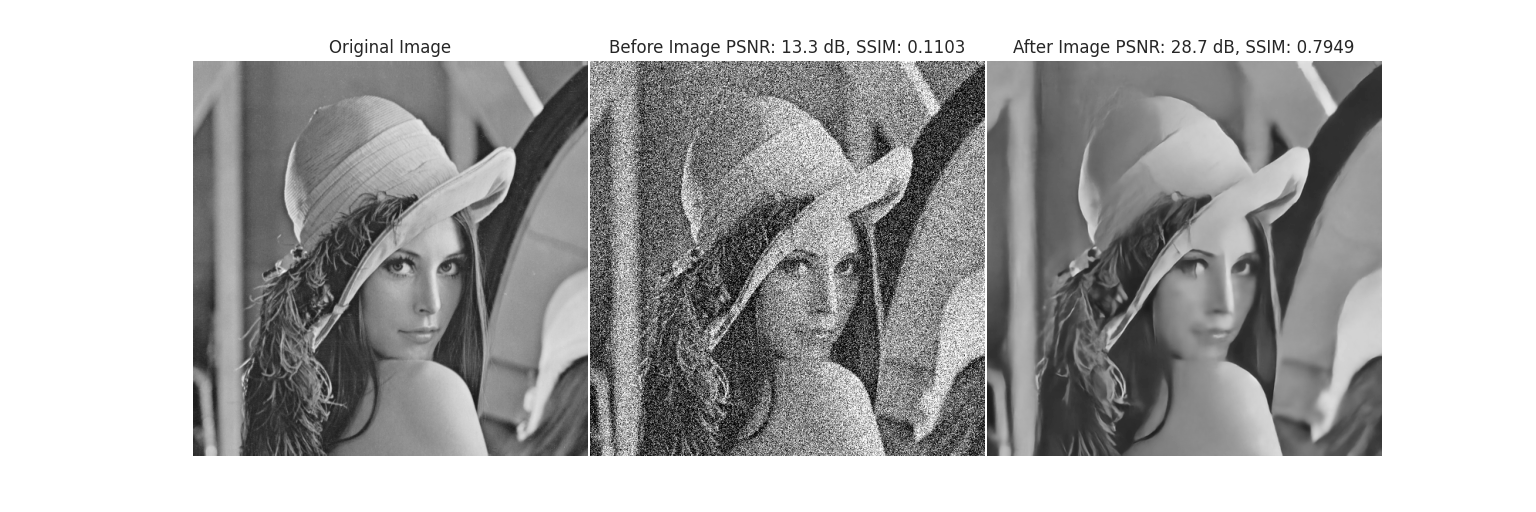
\includegraphics[width=\textwidth]{assets/60_gau_restormer.png}
        \caption{Restormer (Gaussian, 60/250)}
    \end{subfigure}
    \begin{subfigure}{0.48\textwidth}
        \centering
        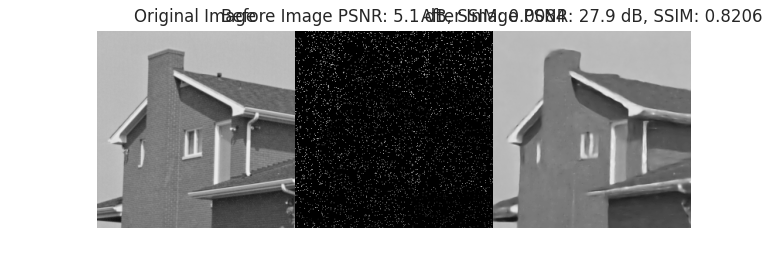
\includegraphics[width=\textwidth]{assets/240_bern_saltnet.png}
        \caption{SaltNet (Bernoulli, 240/250)}
    \end{subfigure}
    \hfill
    \begin{subfigure}{0.48\textwidth}
        \centering
        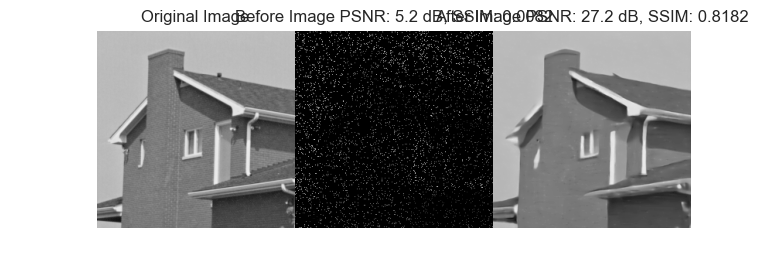
\includegraphics[width=\textwidth]{assets/240_bern_restormer.png}
        \caption{Restormer (Bernoulli, 240/250)}
    \end{subfigure}
    \begin{subfigure}{0.48\textwidth}
        \centering
        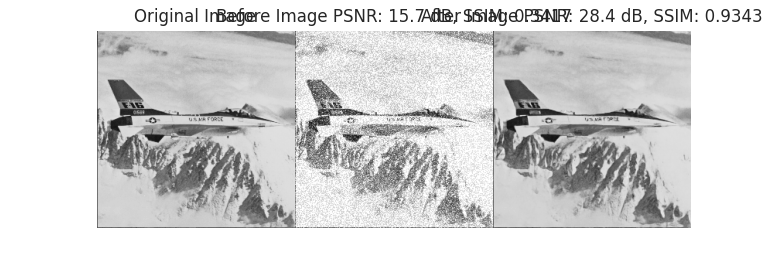
\includegraphics[width=\textwidth]{assets/240_pois_saltnet.png}
        \caption{SaltNet (Poisson, 240/250)}
    \end{subfigure}
    \hfill
    \begin{subfigure}{0.48\textwidth}
        \centering
        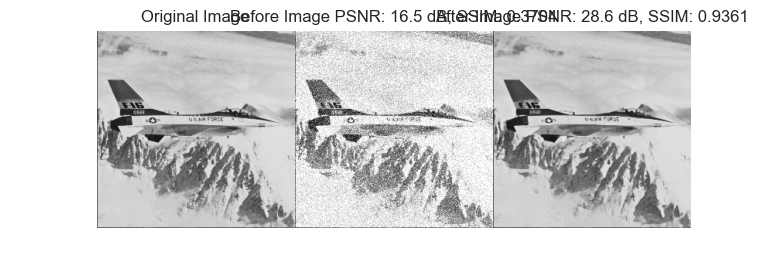
\includegraphics[width=\textwidth]{assets/240_pois_restormer.png}
        \caption{Restormer (Poisson, 240/250)}
    \end{subfigure}
    % \begin{subfigure}{0.48\textwidth}
    %     \centering
    %     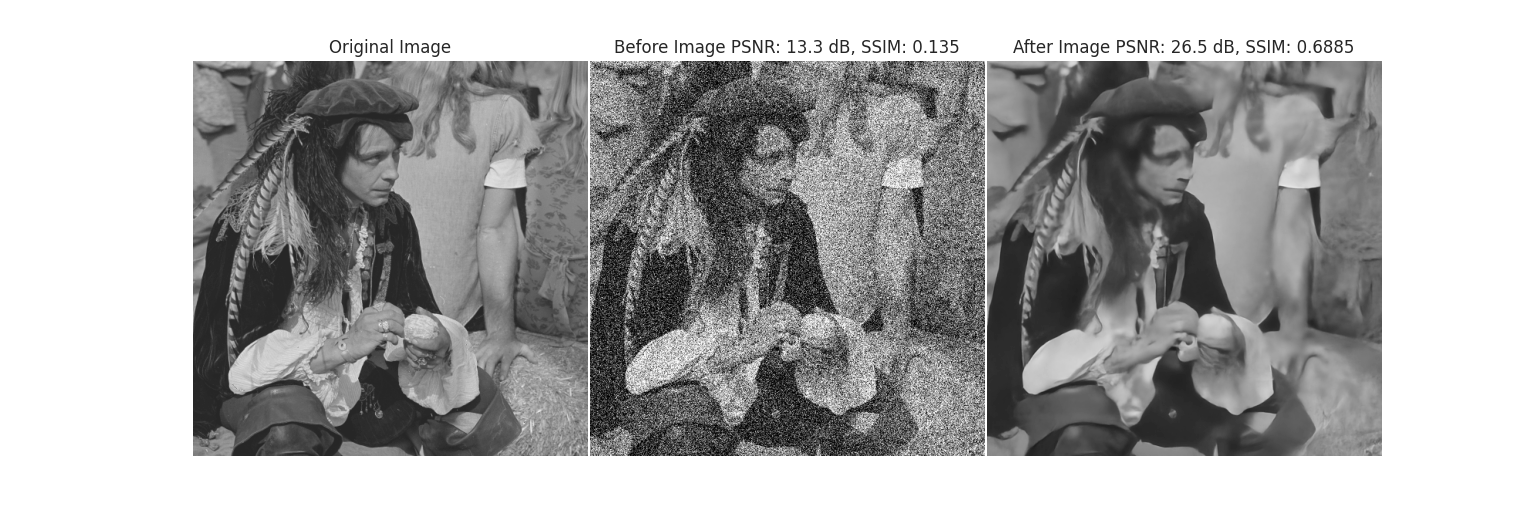
\includegraphics[width=\textwidth]{assets/60_gau_3_saltnet.png}
    %     \caption{SaltNet (Gaussian, 60/250)}
    % \end{subfigure}
    % \hfill
    % \begin{subfigure}{0.48\textwidth}
    %     \centering
    %     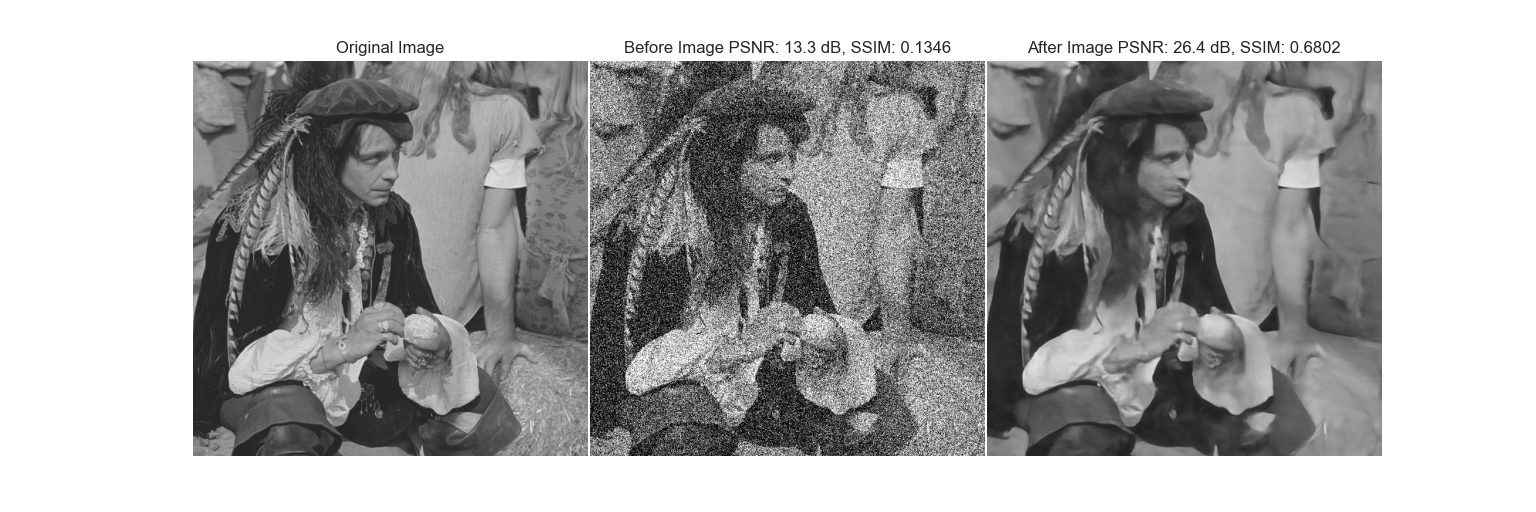
\includegraphics[width=\textwidth]{assets/60_gau_3_restormer.png}
    %     \caption{Restormer (Gaussian, 60/250)}
    % \end{subfigure}
    % \begin{subfigure}{0.48\textwidth}
    %     \centering
    %     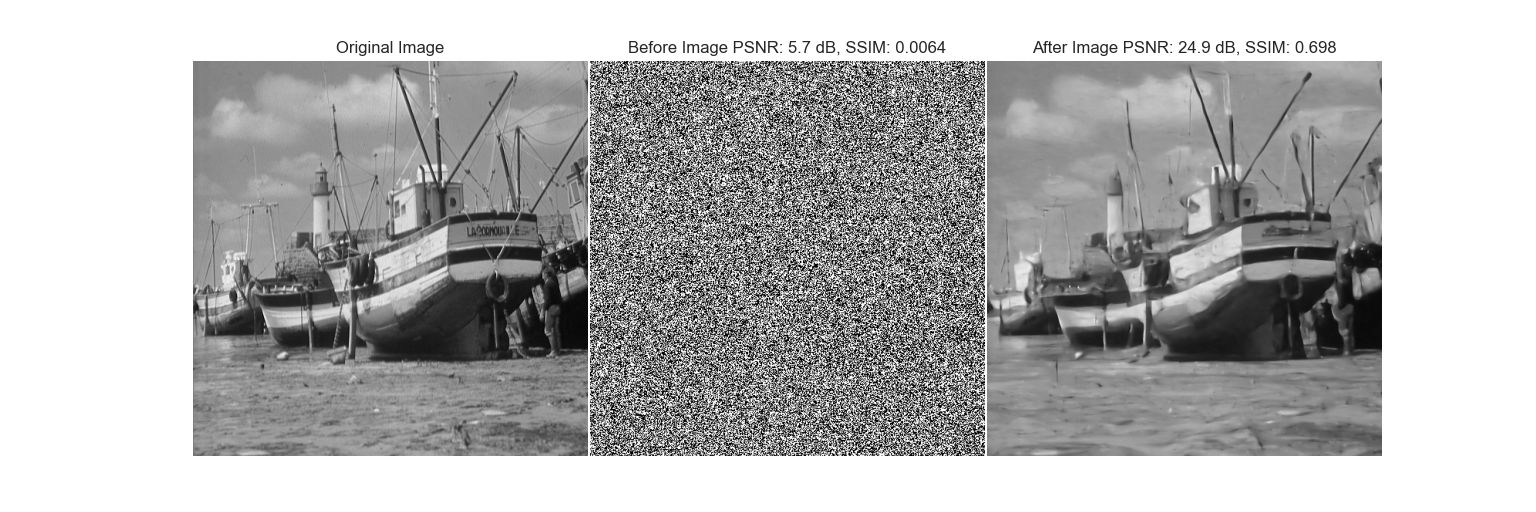
\includegraphics[width=\textwidth]{assets/240_sap_2_restormer.png}
    %     \caption{SaltNet (Salt \& Pepper, 240/250)}
    % \end{subfigure}
    % \hfill
    % \begin{subfigure}{0.48\textwidth}
    %     \centering
    %     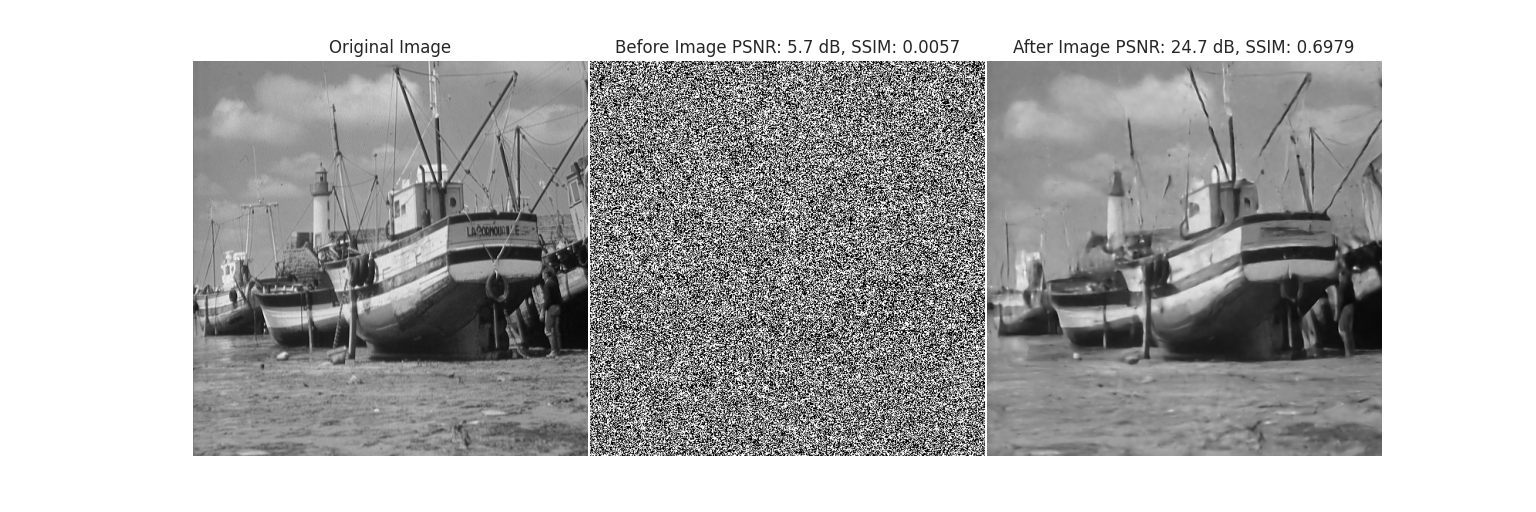
\includegraphics[width=\textwidth]{assets/240_sap_2_saltnet.png}
    %     \caption{Restormer (Salt \& Pepper, 240/250)}
    % \end{subfigure}
    % \caption{Qualitative Results}
\end{figure}

\pagebreak

\subsection{Performance Comparisons}

SaltNet is shown through the results below to be much more resource efficient than Restormer.

\begin{table}[!hbt]
    \centering
    \caption{Performance Comparison}
    \begin{tabular}{lcccccc}
    \toprule
    Size & Restormer Mem. & Our Model Mem. & Restormer Thr. & Our Model Thr. \\
    (px) & (bytes) & (bytes) & (im/s) & (im/s) \\
    \midrule
    64 & 2.60E+08 & 2.23E+08 & 25.15 & 45.27 \\
    128 & 3.22E+08 & 1.43E+08 & 24.12 & 43.95 \\
    256 & 5.45E+08 & 3.22E+08 & 21.42 & 41.60 \\
    512 & 1.77E+09 & 1.04E+09 & 6.36 & 31.63 \\
    1024 & 6.74E+09 & 3.90E+09 & 1.22 & 23.61 \\
    2048 & 1.53E+10 & OOM & OOM & 2.52 \\
    4096 & OOM & OOM & OOM & OOM \\
    \bottomrule
    \end{tabular}
\end{table}

\begin{figure}[!hbt]
        \centering
        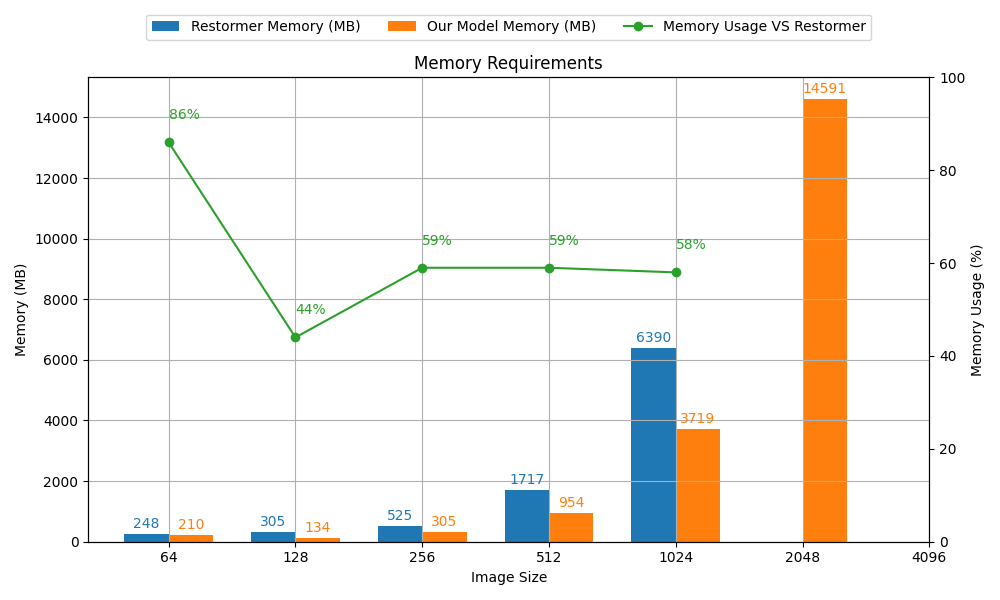
\includegraphics[width=\textwidth]{assets/memory-requirements.png}
        \caption{SaltNet (Poisson, 240/250)}
\end{figure}
\begin{figure}[!hbt]
        \centering
        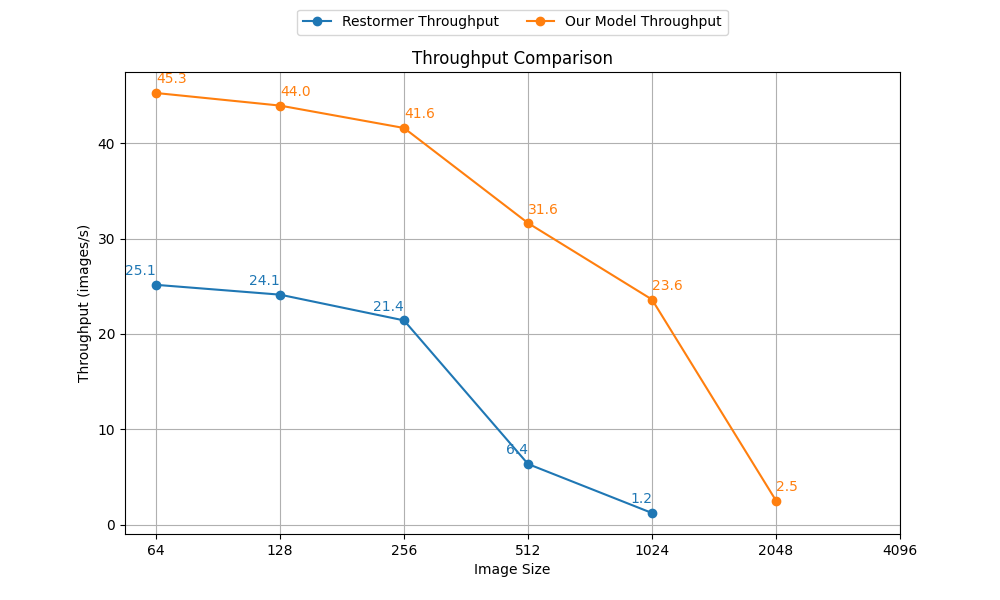
\includegraphics[width=\textwidth]{assets/throughput.png}
        \caption{Restormer (Poisson, 240/250)}
\end{figure}